
Throughout this chapter,
    reference is made to the `Stonehaven Region'.
This is defined as +/- 50km of the crash location for radar data,
    which uses an ordinance survey grid,
    and as +/- 0.5 degrees of the crash location for the radar data.

\section{Empirical Data}\label{sec:def}

The data used in this section is taken from the Met Office's NIMROD system~\cite{radar_data}.
This data has a 5km by 5km spatial resolution and a 15-minute temporal resolution,
    although data is also available in a 1km by 1km spatial resolution.
The coarser dataset was chosen as the Stonehaven event was a Summer convective storm,
    which occurs on scales great enough to be captured at a 5km resolution.

\subsection{The Stonehaven Event}\label{subsec:actualevent}

\subsubsection{Rainfall at the crash location}

\begin{figure}[H]
    \begin{center}
    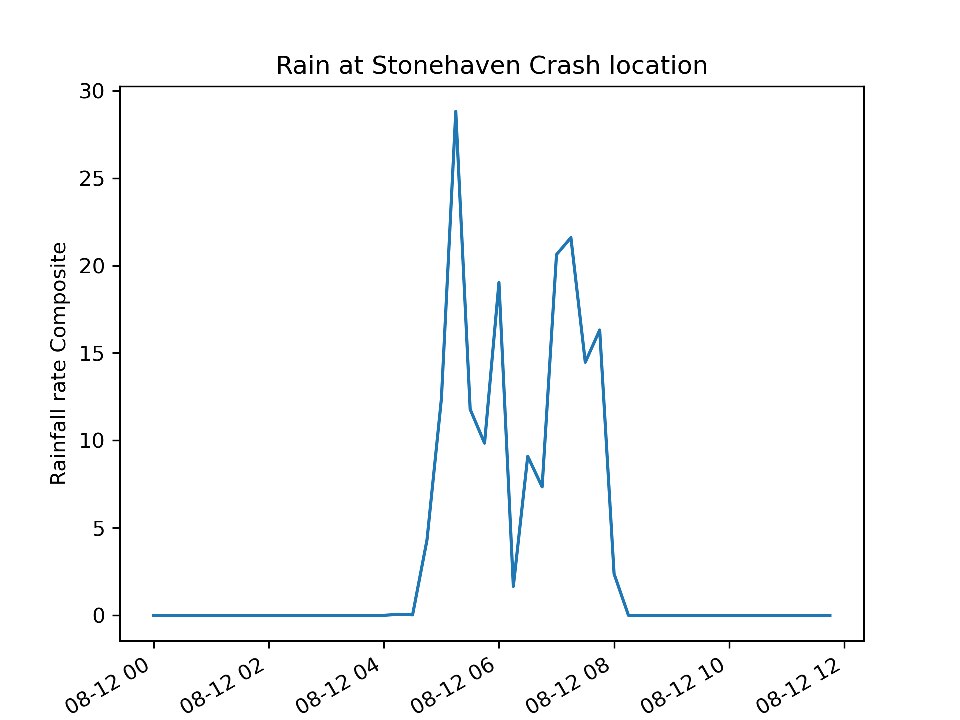
\includegraphics[width=100mm]{stonehavendayraingraph}
    \end{center}
    \caption{A graph of the rainfall at the Stonehaven crash location.
    X-axis is the date and hour (24-hour clock) of the rainfall measurement,
        ranging across the morning of the 12th of August 2020.
    Y-axis is the rainfall measured in mm/h.}
    \label{fig:stonehavendayraingraph}
\end{figure}

From figure~\ref{fig:stonehavendayraingraph},
    the rainfall event begins at 4:15 and ends at 8:15.
The rainfall at the crash location is then given in sixteen 15-minute chunks of time,
    or as across four hours.

This may suggest a four-hour event definition should be used.
However, this was not done for two reasons.
First, it is clear that the rainfall occurred in two 2-hour peaks,
 so a 4-hour definition would not be appropriate for this event.
Second, in section~\ref{subsec:radarprocess},
    the radar data is processed into chunks,
    each of which start on an increment of the length of time of the event.
While this would accurately capture this 4-hour storm, being between 4:00 and 8:00,
    an event from 6:00 to 10:00 would be considered two events of half the size.

A one-hour peak was then used instead.
This was as it allowed storms of a similar length to be quantified by their peak rainfall.

\subsubsection{Rainfall in the Stonehaven region}

\begin{figure}[H]
    \centering

    \begin{subfigure}{0.48\textwidth}
        \centering
        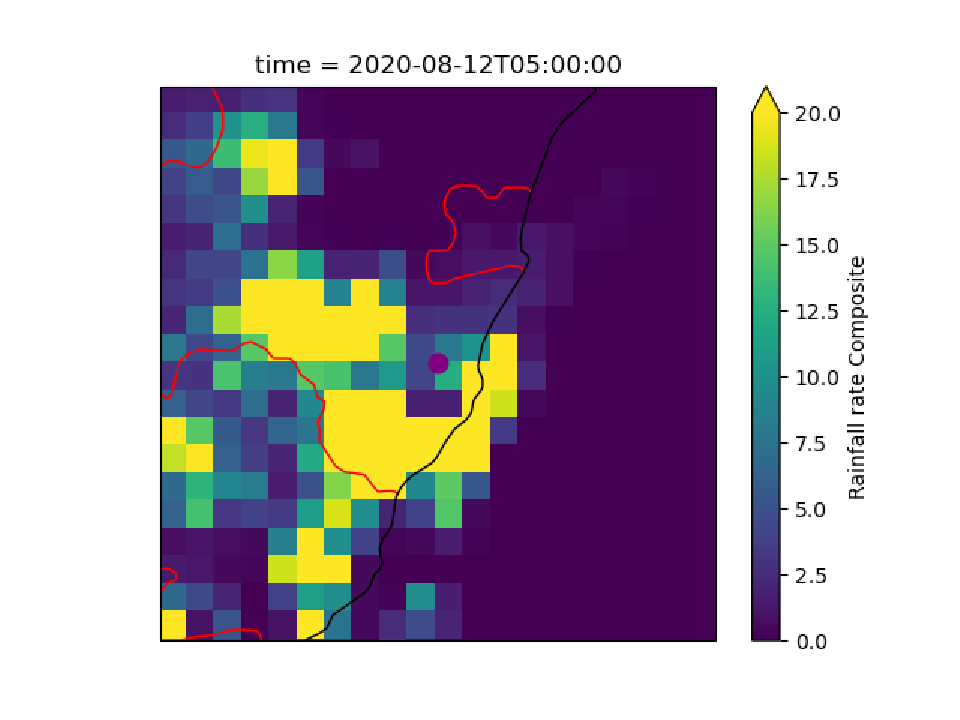
\includegraphics[width=\linewidth]{stonerain5}
    \end{subfigure}
    \hfill
    \begin{subfigure}{0.48\textwidth}
        \centering
        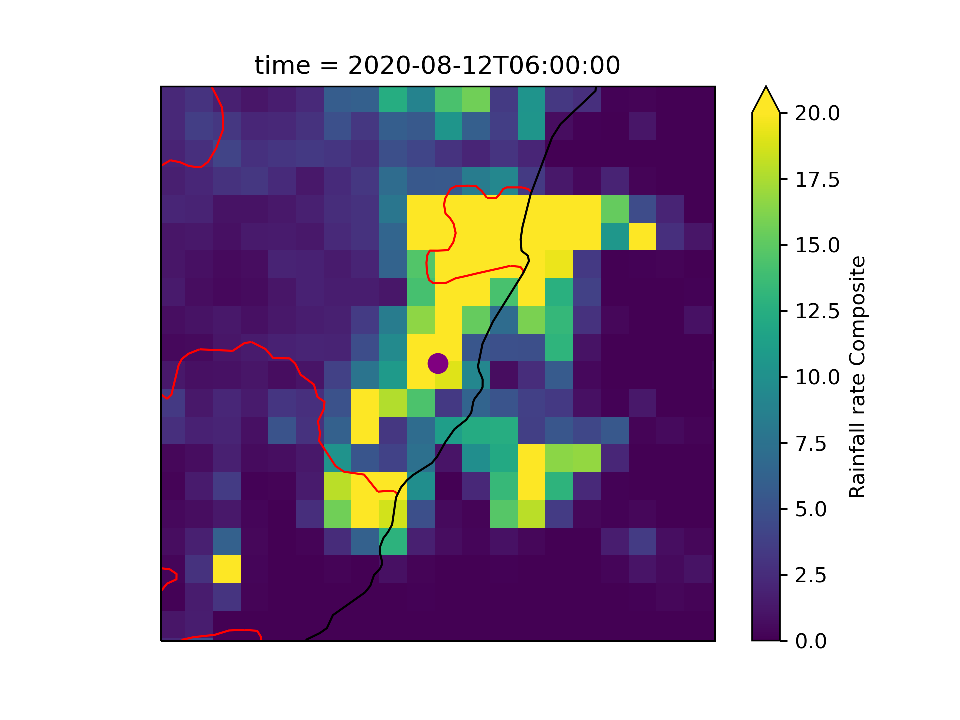
\includegraphics[width=\linewidth]{stonerain6}
    \end{subfigure}

    \vspace{\baselineskip}

    \begin{subfigure}{0.48\textwidth}
        \centering
        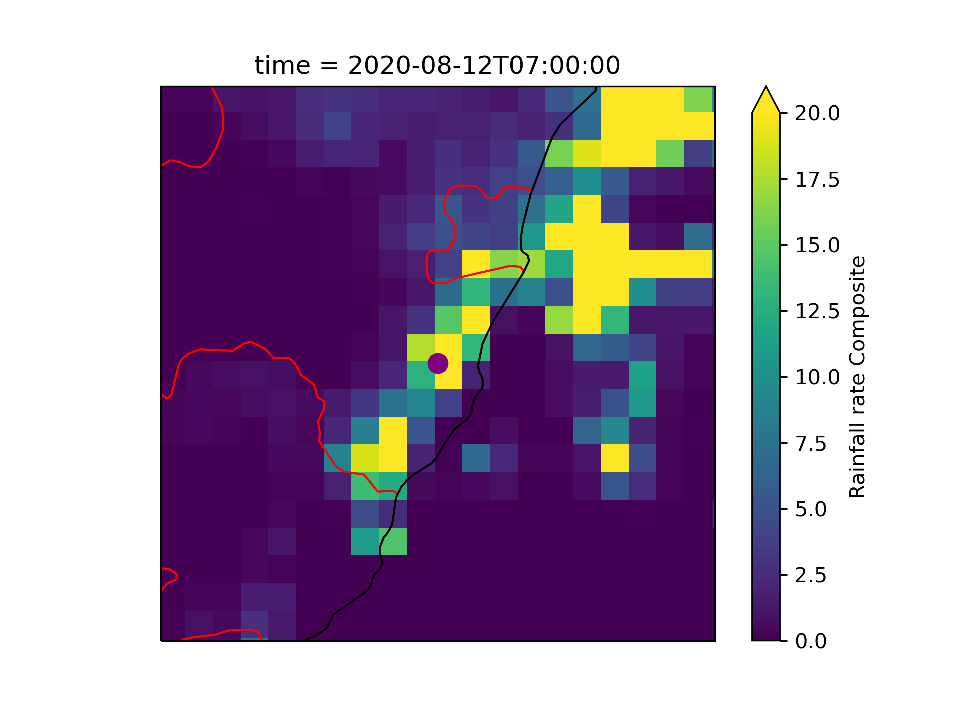
\includegraphics[width=\linewidth]{stonerain7}
    \end{subfigure}
    \hfill
    \begin{subfigure}{0.48\textwidth}
        \centering
        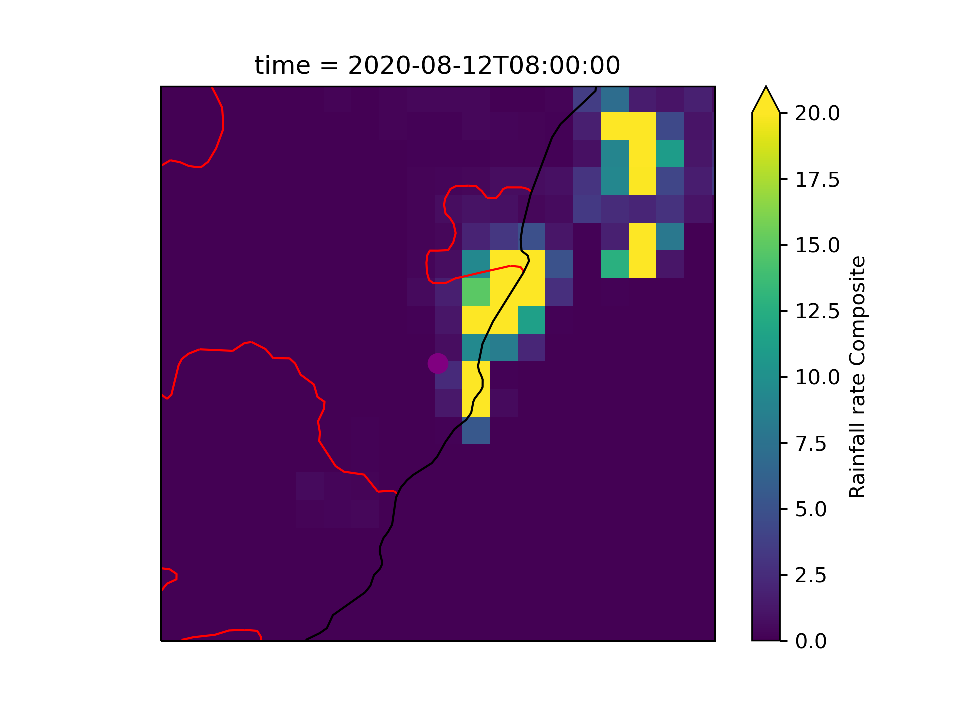
\includegraphics[width=\linewidth]{stonerain8}
    \end{subfigure}
    \caption{Rainfall in the Stonehaven region (+/- 50km of Stonehaven)
        at times of 5, 6, 7 and 8AM of the 12th August 2020,
        in the top left, top right, bottom left and bottom right respectively.
    Scale is mm/h.
    Black lines are coastlines, red lines are local authority boundaries.
    Purple dot is the crash location.}
    \label{fig:stoneregionrain}
\end{figure}

Figure~\ref{fig:stoneregionrain} shows the rainfall in the Stonehaven region,
    demonstrating the movement of the storm North-East throughout the morning of the event.
This figure is also available as an animation using data from 15-minute intervals,
    showing the storm moving as expected.

The figure also suggests that the event covers a large area,
    validating the use of the coarser-resolution 5km dataset as sufficient to describe the event.
One unfortunate consequence of using the 5km dataset is on the rainfall described in figure~\ref{fig:stonehavendayraingraph},
    as the crash location lies near the boundary of four cells, yet the data is only taken from the nearest cell,
    leading to the graph being less accurate approximation of the rainfall at the crash location than would be given by a 1km resolution dataset.

\subsection{Further Constraints}\label{subsec:furthercons}

\subsubsection{Stonehaven Geography}

\begin{figure}[H]
    \centering
    \begin{subfigure}{0.48\textwidth}
        \centering
        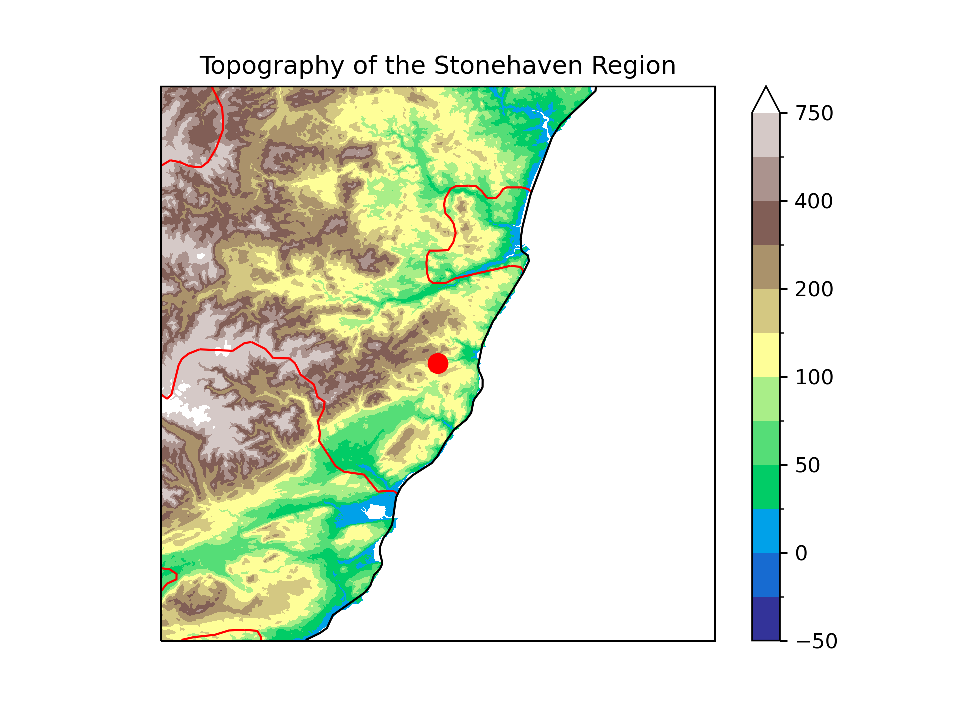
\includegraphics[width=\linewidth]{stonetopog90}
    \end{subfigure}
    \hfill
    \begin{subfigure}{0.48\textwidth}
        \centering
        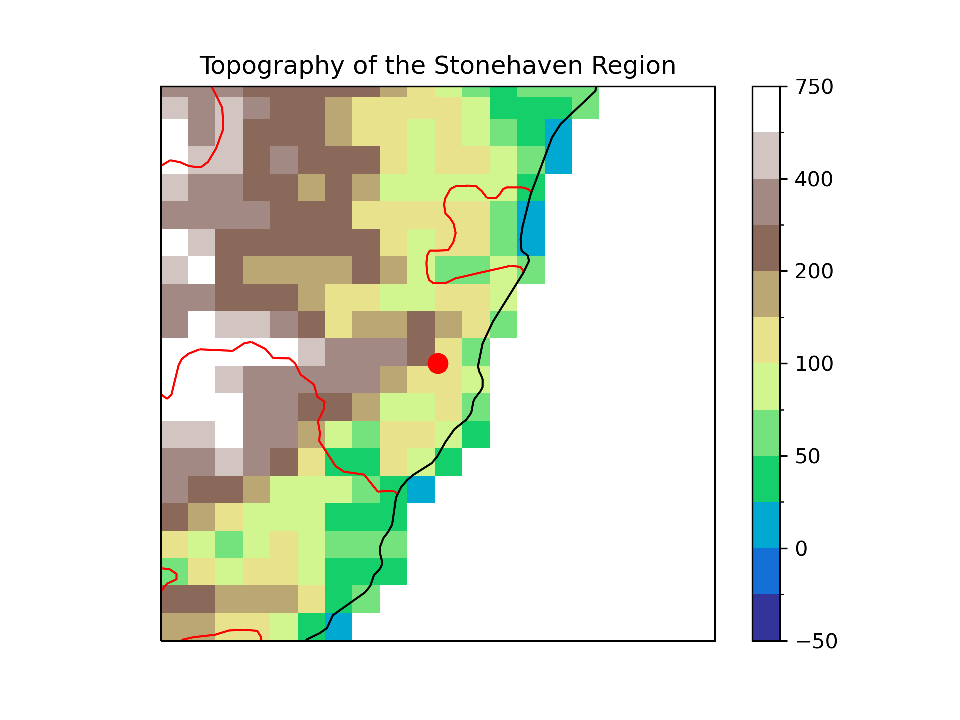
\includegraphics[width=\linewidth]{stonetopog4950}
    \end{subfigure}
    \caption{Plot of the topography in the Stonehaven region.
    Scale is in meters.
    Left is the raw data (at 90mx90m resolution),
    right is the resampled data (at 4950mx4950m resolution) as used for future processing.
    Black lines are coastlines, red lines are local authority boundaries.
    Red dot is the crash location.}
    \label{fig:stonetopog}
\end{figure}

The 4950m resolution data shown in figure~\ref{fig:stonetopog} was found by taking a mean average of 55 of the data points in each dimension,
    giving each grid cell an average of 3250 raw data points.

The area of the Stonehaven crash is around the 200m contour,
    with the crash occurring at around 100m,
    due to the cutting the railway passes through.
Looking at figure 26 of~\cite{RAIB_2022},
    the drain responsible for the crash is 150m above sea level.
Furthermore, the drain's catchment reaches close to 200m.

The topography of the region for the event attribution analysis was then chosen to be from 0m (sea level),
    to 400m.
This is done to make the topography around the crash location typical for the region in which the analysis is performed.
A 200m limit was suggested,
    to match the limit taken in~\cite{Tett_Soon},
    but was not taken forward as this had the potential to give too few data points to define an event.

\begin{figure}[H]
    \begin{center}
        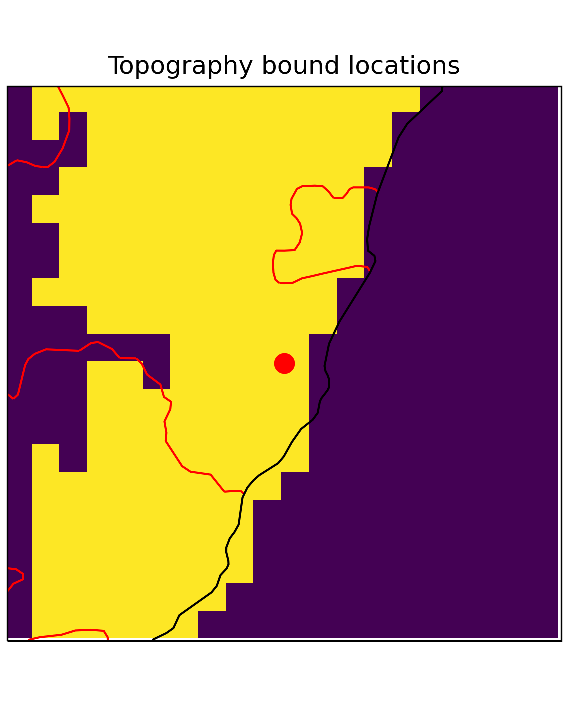
\includegraphics{stonetopogcut}
    \end{center}
    \caption{Map of the Stonehaven region with radar data grid cells (5kmx5km) within a topographical range of 0--400m in yellow,
    grid cells outside of range in violet.
    Black lines are coastlines, red lines are local authority boundaries.
    Red dot is the crash location.}
    \label{fig:stonetopogallowed}
\end{figure}

Out of the 400 grid cells in the Stonehaven Region,
    data is taken from 185 of the grid cells.
This is as 194 of the grid cells are not over land,
    and an additional 21 grid cells have too high topography.

As the radar data is at a 5km resolution,
    while the resampled topography data is at a 4950m resolution,
    the XArray \texttt{interp\_like} method is used to get a linear interpolation for the height at each 5km grid cell.

\subsection{Processing and Fitting the Radar Data}\label{subsec:radarprocess}

The steps used in this section are identical to those used to processing and fitting the radar data for the Edinburgh cloudburst event~\cite{Tett_Soon},
    with changes made to fit the different definition and region in this case.

\subsubsection{Computing Maxima}

As the goal was to use an Extreme Value distribution to model the data,
    it is necessary to draw the extrema out from the data.
The dataset itself~\cite{radar_data} is composed of \texttt{.tar} files, each of which containing the radar data of a given day.

The \texttt{process\_radar\_data} Python script finds the maximum one-hour rainfall in each of these daily datasets and
    uses these to generate a dataset with the one-hour maximum rainfall and the time of the one-hour maximum rainfall
    at all points in the Stonehaven Region for a given month, in a NetCDF format
The \texttt{combine\_summary} Python script then takes these monthly maxima and their times and combines them into a single dataset,
    again as a NetCDF .

These Python scripts are called by the Shell scripts \texttt{run\_jobs} and \texttt{run\_combine} respectively.
The Shell scripts are run on a JASMIN Science Analysis Server and submit the Python scripts as SLURM jobs to the LOTUS Batch Processing Cluster,
    allowing all the monthly maxima to be computed in a single script and the combination of the datasets to access an amount of memory to make the task feasible.

The \texttt{get\_radar\_data} function in the \texttt{stonehavenRainLib} Python script then selects the summer months and
    combines them to get the maximum hourly rainfall in the summer of each year,
    along with the time of the maxima.
This function also applies the topographical height mask described in subsection~\ref{subsec:furthercons},
    returning an XArray DataSet of the radar data that will be used to describe and generate statistics for the event.

\subsubsection{Computing Events and Definition}

Now that the seasonal maxima have been found,
    the data can be used to define events.
This process is done in the \texttt{gen\_radar\_data} function in the \texttt{stonehavenRainLib} Python script.
The seasonal maxima,
    of which there is one for each grid cell in each year in the dataset,
    are grouped by the time in which they occurred.

These groups are 12-hour periods,
    representing either the AM or PM hours of a day.
Each group is then an event,
    containing the grid cells which experienced their maximum hourly rainfall within the group's time period.
The groups with less than 10 grid cells were discarded,
    as these events are less than 250km$^2$ in size and
    so do not represent events similar enough to the Stonehaven event.

This gives a final event definition as 250km$^2$ of the land below 400m and within +/- 50km of Stonehaven
    experiencing their annual summer hourly rainfall maxima in the same 12-hour period.
For each event, the 0.05, 0.1, 0.2, 0.5, 0.8, 0.9 and 0.95 quantiles were found and returned in a dataset.
The intensity of a given event is defined by its 0.95 quantile.

Due to the separation into 12-hour bins,
    it is assumed that each event is independent in all future calculations.

\begin{figure}[H]
    \centering
    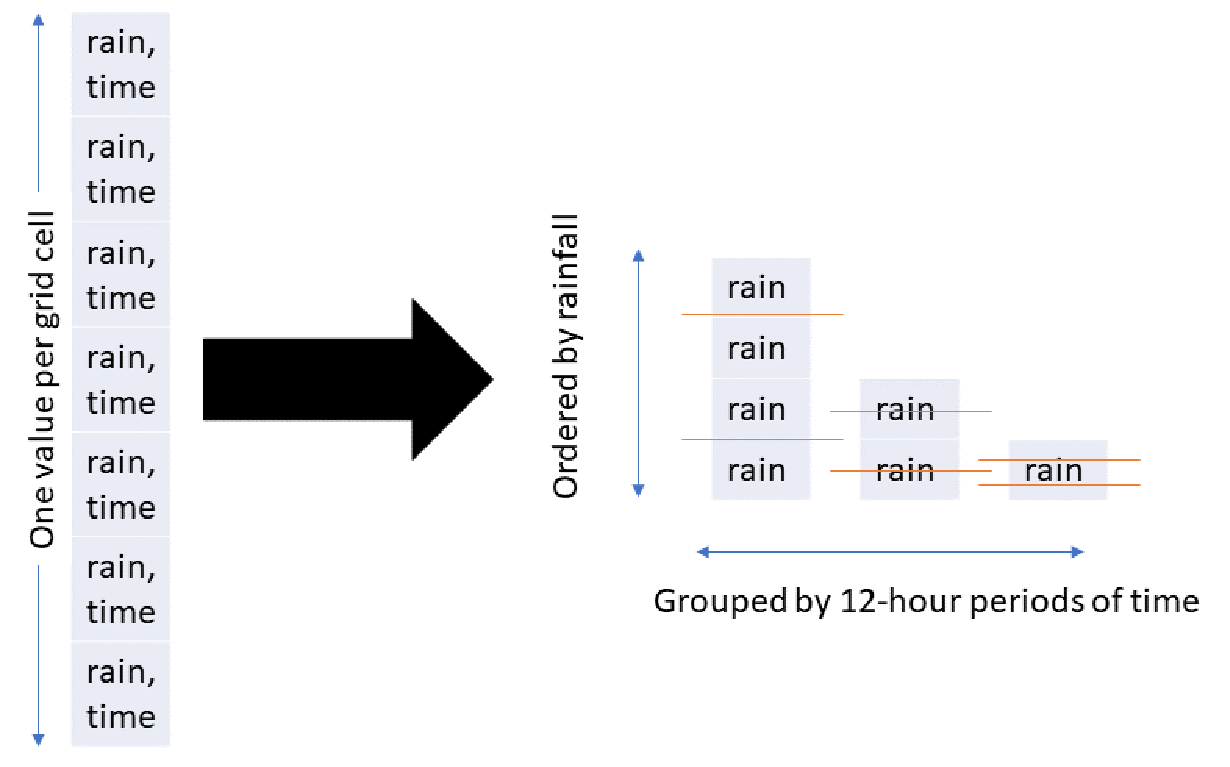
\includegraphics[width=80mm]{dataprocessschematic}
    \caption{Diagram representing the data processing after the maxima of each grid square has been found,
    within each year.
    `rain' represents the summer maximum rainfall in a grid cell,
        `time' represents the time of this maximum,
        red horizontal lines represent the taking of quantiles from the rainfall maxima.
    Number of data points and quantiles are not to scale.}
    \label{fig:dataprocessschematic}
\end{figure}

\subsubsection{Fitting event distribution}

The radar data is fit to a GEV distribution with the \texttt{comp\_radar\_fits} Python script,
    which calls the \texttt{gev\_r} Python library to run code in R .
The `fevd', fit extreme value distribution,
    command in R is used to fit an extreme value distribution to the radar data,
    which uses MLE, as described in subsection~\ref{subsec:parameterest}.
This command is applied each of the quantiles of the event,
    with the events as the data points,
    giving the parameters of GEV distributions describing each quantile of the events.
With these parameters generated,
     it was possible to find the empirical return period for the Stonehaven event.

To generate uncertainties,
    a Monte Carlo bootstrap method is used,
    given in the \texttt{mc\_dist} function.
This involved generating a list of the same size of the number of events,
    taking a random sample with replacement,
    then applying the `fevd' command to each sample.

1000 samples were taken,
    of which 9 provided anomalous (negative) location or scale parameters,
    and so were discarded.
The discarding process was valid as the value of these parameters was ~-100,
    while all other samples had values of these parameters between 2 and 15,
    as well as that removing this few samples would not have a significant effect on the 95\% confidence interval.
The 991 samples left are greater than the 800 suggested by Booth and Sarkar~\cite{Booth_Sarkar_1998}
    for an effective error estimation.

\section{Modelled Data}\label{sec:model}

The model data used in this section is
    the Met Office Hadley Centre's UKCP18 Convection-Permitting Model Projections for the UK at 2.2km resolution~\cite{model_data}.
This dataset was chosen as the resolution is less than 5km,
    and so is able to accurately represent convective storms.

The CPM ensemble consists of 12 members and covers the 100 years from 1981 to 2080,
    modelling the RCP8.5 emissions scenario.
In this investigation,
    the model's hourly temperature and rainfall data will be used

\subsection{Pre-processing}\label{subsec:preprocess}

The CPM data used is on longitude-latitude coordinates,
    with a north pole rotated to near the region the model covers.
The location of the Stonehaven crash in this alternative coordinate system was found using the \texttt{comp\_rotated\_coords} Python script,
    using CartoPy for the computations.
This coordinate rotation was also done for the four weather stations used to compute Central England Temperature (CET).

The pre-processing of the CPM data is done using the \texttt{ens\_seas\_max\_coarsen} python script,
    which finds the seasonal one-hour rainfall maxima for each grid cell.

\subsubsection{Coarsening}

The CPM data uses a 2.2km resolution,
    while the radar data uses a 5km resolution.
To account for this,
    the radar data is coarsened using the XArray \texttt{.coarsen} and \texttt{.mean} methods,
    taking the mean average of four 2.2kmx2.2km grid cells, giving 4.4kmx4.4km grid cells.

The height mask for the CPM was in the same 2.2km resolution
    and so required the same pre-processing

\subsubsection{Height mask}

To match the event definition in section~\ref{subsec:radarprocess},
    a similar height mask must be used,
    with the same limits of 0m to 400m.

The CPM used for this study is a projection over land,
    with other UKCP18 models covering the marine domain,
    albeit at a lower resolution of 12km and covering storm surges and sea levels as opposed to precipitation,
    as described in the guidance of~\cite{model_data}.
This makes the >0m height mask on the model a necessity,
    as the model projections over the sea (with height 0m) are invalid.

\subsection{Covariates}\label{subsec:covfit}

\subsubsection{Time Series}

The \texttt{comp\_cpm\_ts} Python script was used to compute the time series.
This script takes each month in each ensemble member the CPM data and computes 3 values.
These are computed using the 2.2km data without the coarsening or height mask.
First is the Central England Temperature,
    which takes the CPM data's average monthly temperature at the weather stations used to define CET,
    while the other two time series use the average monthly temperature and precipitation in the Stonehaven Region.

Two additional monthly time series were computed in the \texttt{analyse\_cpm\_data\_rolling} Python script.
One of these takes the median extreme precipitation across the Stonehaven Region
    using the extrema processed in \texttt{ens\_seas\_max\_coarsen.sh},
While another uses the temperature in the Stonehaven Region to find the Saturation Specific Humidity.

The formula used for this is the August-Roche-Magnus approximation to the Clausius-Clapeyron relation~\cite{Alduchov_Eskridge_1996}, given by:
\begin{equation}\label{eq:qsat}
    e_s = 6.112 \exp\left( \frac{17.6 T}{T + 243.5} \right)
\end{equation}
Where $T$ is the temperature in degrees Celsius.

The scaling of the Saturation Specific Humidity with temperature will be described as the Clausius-Clayperon scaling.
This is as it represents the amount of moisture that the atmosphere can hold,
    suggesting that rainfall should also scale by this amount with a change in temperature.

Each time series had 14400 members,
    with 12 ensemble members providing data for the 1200 months across the 100-year window of the model.
This was then reduced to 3600 data points by only taking the three summer months of each year.

\subsubsection{Fitting Covariates}

\texttt{analyse\_cpm\_data\_rolling} performs a linear fit of the Saturation Specific Humidity,
    Stonehaven Region temperature, mean average Stonehaven Region precipitation and mean maximal Stonehaven Region precipitation.
    using the \texttt{statsmodels} Python package's ordinary least squares regression feature.
This provides the change in each of these variables, as well as the uncertainty with $R^2$ coefficients,
    with respect to each fit.

In a method analogous to the \texttt{comp\_radar\_fits} Python script calling the \texttt{gev\_r} library to use R to fit
    a distribution to the radar rainfall extrema in subsection~\ref{subsec:radarprocess},
    \texttt{analyse\_cpm\_data\_rolling} calls the \texttt{gev\_r} library to perform fits on the model rainfall extrema.
This is done with the same `fevd' command in the extRemes R library~\cite{extremes_R},
    except done with the monthly mean CET, total model area temperature, Stonehaven Region temperature and Stonehaven Region humidity as covariates.

For this,
    the location and scale parameters are allowed to change linearly with the variable $x$.
The parameters are then $\mu = \mu_0 + x\mu_1$ and $\sigma = \sigma_0 + x\sigma_1$.
The analysis is then repeated with the shape parameter also allowed to vary in the form $\xi = \xi_0 + x\xi_1$.

In contrast to \texttt{comp\_radar\_fits},
    \texttt{analyse\_cpm\_data\_rolling} does not perform a single GEV fit on a set of events,
    but instead a GEV fit for each grid cell in the Stonehaven region for the CPM .
This far greater number of fits is possible as the CPM data contains data for 1200 summer maxima for each point,
    with each of the 12 ensembles spanning 100 years,
    as opposed to the 16 for the radar data.
A data fit for each grid cell then allows the effect of the location on the CPM rainfall maxima to be analysed.
This data fit is done nine times,
    with either no covariate or the CET, CPM Region temperature, Stonehaven Region temperature or Stonehaven Region saturated humidity as a covariate.
For each covariate, this is performed with and without the shape parameter varying.

The scaling of the parameters $\mu_1 / \mu_0$, $\sigma_1 / \sigma_0$ and, where the shape is also fit to the covariate,
    $\xi_1 / \xi_0$ can then be found at each grid cell.
These fits and scalings are also computed for the 2 hour, 4 hour and 8 hour summer rainfall maxima.

For the CET fit,
    confidence intervals in these scalings are found using a Monte Carlo bootstrap method.
This takes a random sample, with replacement, of 1\% of the grid cells and takes the mean of the scaling that sample,
    with the small sample size allowing the assumption of the samples being independent.
The quantiles of the 1000 samples taken are then used as confidence intervals.
Both the bootstrap sample means and overall mean of the scalings are saved to be used in the risk ratio calculation.
The overall mean scalings will be considered as simply the model scalings in later steps in the development.

These scalings can be compared to the scaling expected from the Clausius-Clapeyron relationship,
    which is computed by taking the linear fit of $H = H_0 + xH_1$ and computing $H_1 / H_0$.
This is a valid comparison, as if the rainfall maxima is given by the CDF~\ref{eq:gevcdf},
    then the distribution of the rainfall maxima multiplied by a constant is given by the same CDF,
    with the location $\mu$ and scale $\sigma$ multiplied by the same constant.

For both the linear and GEV fits against CET, the $\alpha_0$ for all parameters $\alpha$ is given by the value of that parameter for
    the mean summer CET from 2012 to 2021.
The covariate $x$ may then be determined as the difference from the CET in a month to the mean summer CET in 2012--2021.

\subsection{Calculating Risk Ratios}\label{subsec:riskratios}

The final calculation steps are performed in the \texttt{plot\_intensity\_risk\_ratios} Python script.
This begins by finding the value of CET in different time periods.
For historical time periods,
    this is recorded by the Met Office~\cite{CET},
    and the summer mean CET is used.
The periods this data is drawn from are 1850--1899 (Pre-Industrial),
    1980--1989, 2005--2020 and 2012--2021.
For the hypothetical 2K warmer than Pre-Industrial word seasonal mean CET,
    the Pre-Industrial CET is increased by 1.88$\pm$0.06 degrees using a normal distribution,
    taking the distribution from~\cite{Tett_Soon}.

\subsubsection{Applying CPM scaling to Empirical Distribution}

Let $T_0$ be the mean summer CET in the 2005--2020 range.
For each temperature, $\delta T$ is computed as $T - T_0$.

The value of a parameter $\alpha$ in the GEV distribution fit to empirical events is then scaled to $\alpha_T$ at the new temperature:
\begin{equation}\label{eq:newradarparams}
    \alpha_T = \alpha + \delta T \frac{\alpha_1}{\alpha_0} \alpha
\end{equation}
Where $\alpha_1$ is the change in the parameter of the distribution of the extreme events in the model with respect to CET and
    $\alpha_0$ is the value of the parameter of the modelled extreme event distribution in the 2012--2021 temperature range.

This process is repeated, once with the shape parameter fixed, only applying the scalings $\mu_1 / \mu_0$ and $\sigma_1 / \sigma_0$
    from the model distribution to the empirical distribution and again also applying the third $\xi_1 / \xi_0$ from the shape covariate fit.
Both of these are repeated four times, using the scalings from the 1, 2, 4 and 8 hour model maxima,
    although only the 1 hour maxima will be used to directly compute any risk ratios.

This changes the empirical event distribution equivalently to the fitting of covariates to the model distribution in subsection~\ref{subsec:covfit},
    as where the model parameters are multiplied by a factor $k$ due to changes in CET,
    the event distribution parameters are assumed to also be multiplied by a factor of $k$.
The key assumption made here is that the processes driving the change in the maxima from the model will act equivalently
    on the extreme events defined in subsection~\ref{subsec:radarprocess}, as discussed in a supplement to~\cite{Tett_Soon}.

\subsubsection{Calculating Ratios}

To calculate the probability ratio for an event of a given intensity $I$,
    the survival function of the distribution at each time period is used to find the probability of finding an event of equal or greater intensity.
$p_0$ is this probability for the distribution in the Pre-Industrial (1850--1899) world,
    with $p_1$ being the survival function value for a given other time period.
The probability ratio for the event of intensity $I$ in the time period is then $p_1/p_0$.

Equivalently, to calculate the intensity ratio for an event with return period $P$,
    the inverse survival function of the distribution at each time period is used to find the event for which the probability of finding an event of equal to or greater intensity is $1/P$.
$I_0$ and $I_1$ are the intensities of the event for the distribution in the Pre-Industrial world and in the given time period respectively,
    with the intensity ratio as $I_1/I_0$.
An intensity ratio expected from Clausius-Clapeyron scaling was also computed directly by allowing the event intensity to scale identically to saturation humidity with temperature.

As both the intensity and the return period of the Stonehaven event are known,
    it is straightforward to calculate these ratios.
The `headline' ratios found in the abstract are those found by applying the 1 hour model maxima scaling to the empirical event distribution.
However, the ratios were also determined for a collection of intensities and return periods to allow the effect of these on the ratio to be plotted.
This is repeated for using fits based on the 1, 2, 4 and 8 hour model maxima.

For the probability and intensity ratios found for the fits based on the 1 hour model maxima,
    comparing Pre-Industrial to a 2K warmer world,
    a Monte Carlo bootstrap is used to find confidence intervals.
This takes \textasciitilde1000 random samples, each taking one element of the set of \textasciitilde1000 empirical fits found from the Monte Carlo process in subsection~\ref{subsec:radarprocess}
    and one element of the set of \textasciitilde1000 CPM scalings found in the Monte Carlo process in subsection~\ref{subsec:covfit}.
Each sample applies its CPM scaling to its Distribution and calculates the risk ratios as described above.
The quantiles of these probability and intensity ratios give the confidence intervals.

The computation of the probability and intensity ratios is repeated with alternative definitions of the intensity of the event
    as each of 0.05, 0.1, 0.2, 0.5, 0.8 and 0.9 quantiles as opposed to the 0.95 quantile from the definition in subsection~\ref{subsec:radarprocess},
    with the emprical fit for each of these quantiles scaled to the 1 hour model maxima,
    to assess the effect of event definition on the outcome of the analysis.
The risk ratio analysis is done twice, once with and once without a covariate fit shape parameter.